\emph{General observations:}\\
Fig. \ref{fig:results_array}. below contains the parameters and global error results of the experiments we made. We monitored the effect of each parameter by changing it slightly from one execution to another. Going in the details of each execution, we will expose in this part the questions they do and do not answer.\\
\begin{figure}
\centering
	\label{fig:results_array}
	\caption{Experiments parameters and $J$ final value.}
	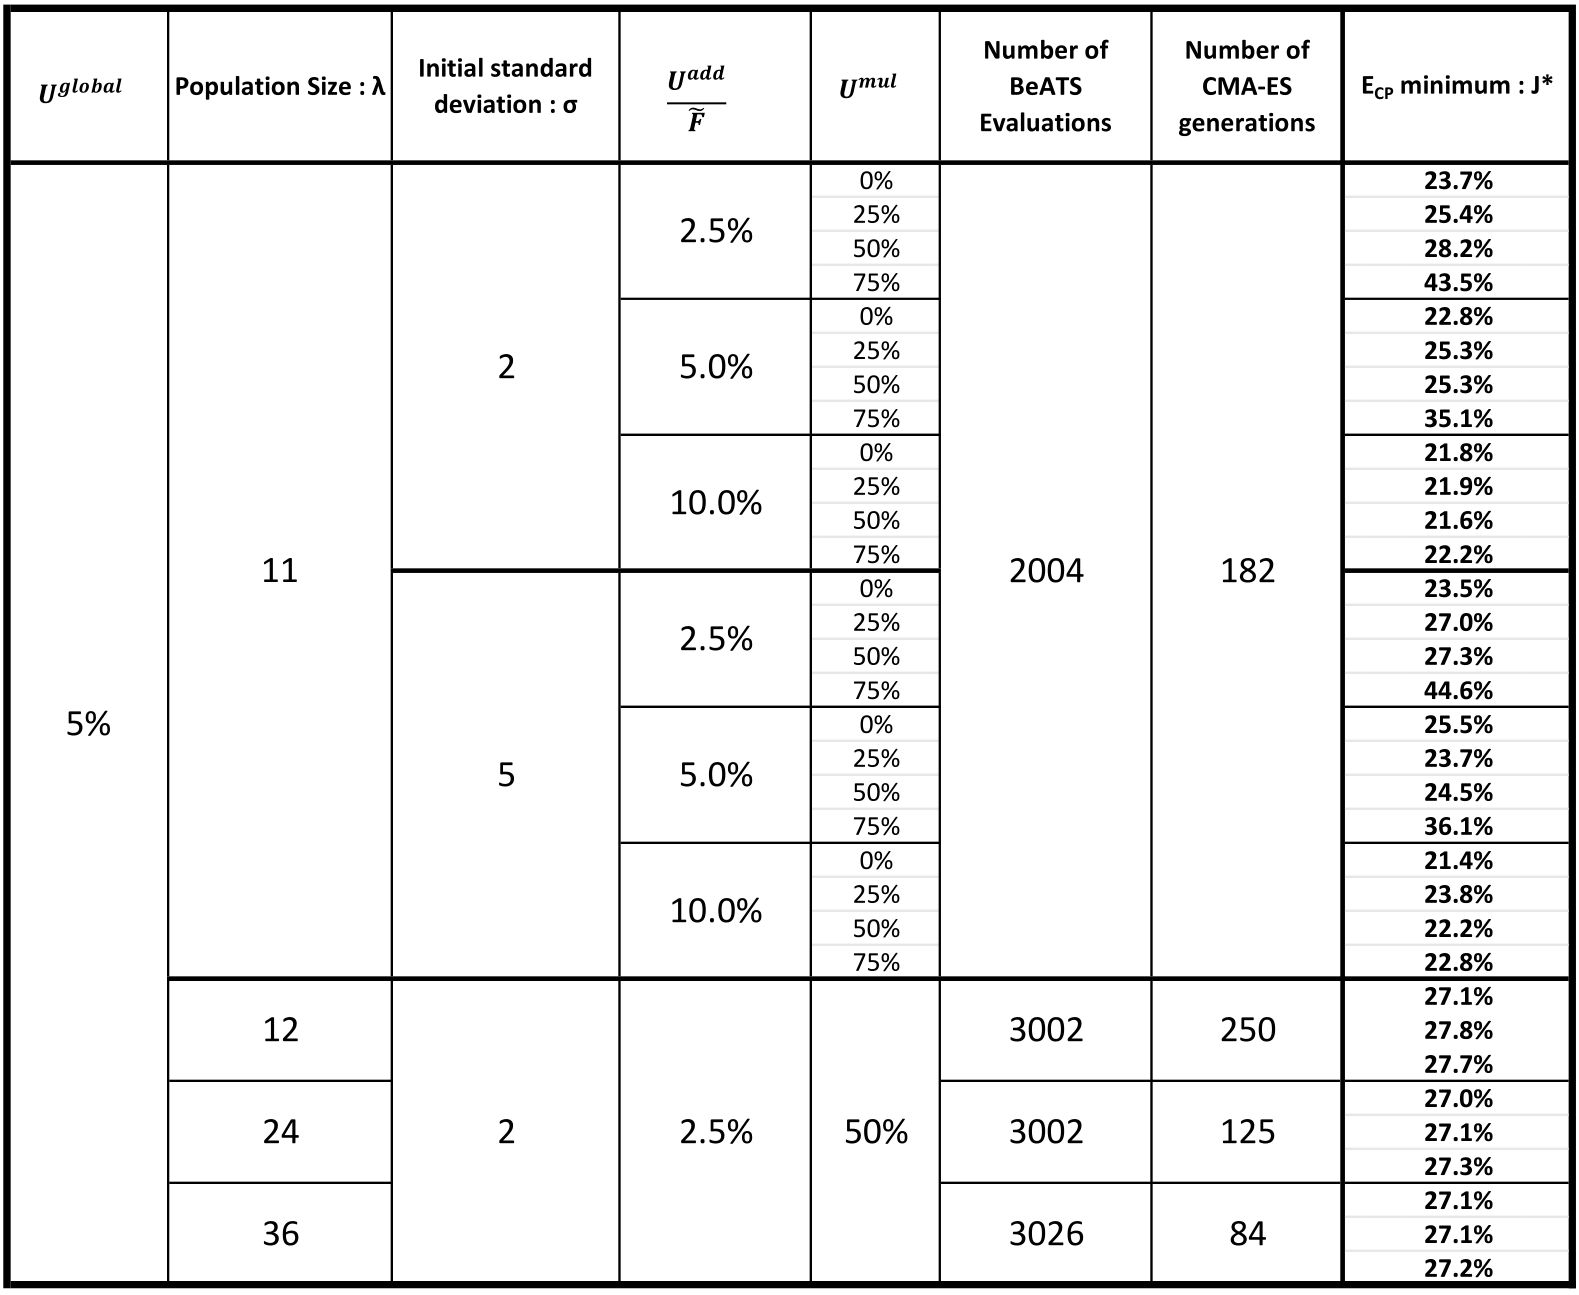
\includegraphics[width=7in]{figures/results_array.png}
\end{figure}
Fig. \ref{fig:results_graph} below displays the influence of the main parameters on $J^{*}$.
\begin{figure}
	\caption{Evolution of $J^{*}$ with the parameters.}
\end{figure}





\begin{enumerate}
	\item Effects of changing the parameters(initial standard deviation, changing the boundaries, changing the weights, changing the uncertainty, changing size of population).
	\item Describe quality and usefulness of the result
	\item Talk about uniqueness. Way to improve (test experiment): increasing population size.\emph{Should we contact the creator of CMAES to ask him about the uniqueness of the solution (i.e. how to improve it ?}
	\item Is our problem "noisy" ?
	\item Talk about how cmaes behaves the way we want
	\item Talk about what happens when we tune also the monitored ramps knobs.	
	\item Talk about issues:
\begin{enumerate}
	\item Limit to result quality due to templates/FDS
	\item Constraints handling has to be improved because several knobs end on their boundaries values\
	\item Uncertainties are symmetric: making them fit the sensors bias (e.g. : if they always under estimate) would be better.
\end{enumerate}
	\item BLABLABLA
\end{enumerate} 
